\documentclass[11pt]{article}

% ============================================================
%  PulseTrace — Investor Deck & Pitch Scripts
%  Compile: pdflatex INVESTOR_DECK.tex  (run twice for refs)
% ============================================================

\usepackage[a4paper,margin=2.1cm]{geometry}
\usepackage[T1]{fontenc}
\usepackage[utf8]{inputenc}
\usepackage[default]{lato}
\renewcommand{\familydefault}{\sfdefault}
\usepackage{amssymb}
\usepackage{pifont}
\newcommand{\cmark}{{\color{ptgreen}\ding{52}}}
\usepackage{microtype}
\usepackage{xcolor}
\usepackage{booktabs}
\usepackage{array}
\usepackage{tabularx}
\usepackage{colortbl}
\usepackage{enumitem}
\usepackage{tikz}
\usepackage{pgfplots}
\usepackage{titlesec}
\usepackage{fancyhdr}
\usepackage{hyperref}
\usepackage{graphicx}

\pgfplotsset{compat=1.17}
\usetikzlibrary{shapes.geometric,arrows.meta,positioning,calc,backgrounds,fit}

% ---------- Brand palette ----------
\definecolor{ptink}{HTML}{0B1220}      % near-black navy
\definecolor{ptpanel}{HTML}{131C2E}    % panel
\definecolor{ptblue}{HTML}{3B82F6}     % primary accent
\definecolor{ptcyan}{HTML}{22D3EE}     % secondary accent
\definecolor{ptgreen}{HTML}{34D399}    % win green
\definecolor{ptred}{HTML}{F87171}      % danger / rival
\definecolor{ptgray}{HTML}{8B98AD}     % muted text
\definecolor{ptline}{HTML}{25324A}     % borders

\hypersetup{colorlinks=true,linkcolor=ptblue,urlcolor=ptblue}

% ---------- Section styling ----------
\titleformat{\section}{\Large\bfseries\color{ptink}}{\thesection.}{0.6em}{}[\vspace{-0.4em}{\color{ptblue}\rule{\linewidth}{1.4pt}}]
\titleformat{\subsection}{\large\bfseries\color{ptblue}}{}{0em}{}
\titleformat{\subsubsection}{\bfseries\color{ptink}}{}{0em}{}

\fancypagestyle{pt}{%
  \fancyhf{}
  \renewcommand{\headrulewidth}{0pt}
  \fancyfoot[L]{\footnotesize\color{ptgray}PulseTrace — Confidential Investor Deck}
  \fancyfoot[R]{\footnotesize\color{ptgray}\thepage}
}
\pagestyle{pt}

% ---------- Helper: callout box ----------
\newcommand{\insightbox}[2]{%
  \begin{tikzpicture}
    \node[draw=ptblue,line width=1pt,rounded corners=4pt,fill=ptpanel!8,
          inner sep=10pt,text width=\linewidth-24pt] (b) {%
      {\bfseries\color{ptblue} #1}\par\vspace{2pt}\color{ptink}#2};
  \end{tikzpicture}\vspace{4pt}}

% ---------- TikZ flow node styles ----------
\tikzset{
  stage/.style={rectangle,rounded corners=3pt,draw=ptline,line width=0.8pt,
                fill=ptpanel!10,minimum height=9mm,inner xsep=6pt,
                align=center,font=\footnotesize\bfseries,text=ptink},
  store/.style={cylinder,shape border rotate=90,draw=ptgreen,line width=0.8pt,
                fill=ptgreen!12,aspect=0.3,minimum height=11mm,minimum width=20mm,
                align=center,font=\scriptsize\bfseries,text=ptink},
  dec/.style={diamond,draw=ptcyan,line width=0.8pt,fill=ptcyan!12,aspect=2,
              align=center,font=\scriptsize\bfseries,text=ptink},
  flow/.style={-{Stealth[length=2.4mm]},line width=0.9pt,draw=ptblue},
  back/.style={-{Stealth[length=2.4mm]},line width=0.9pt,draw=ptred,dashed},
}

\begin{document}

% ============================================================
\begin{titlepage}
\begin{tikzpicture}[remember picture,overlay]
  \fill[ptink] (current page.south west) rectangle (current page.north east);
  % subtle grid
  \begin{scope}
    \clip (current page.south west) rectangle (current page.north east);
    \foreach \y in {0,...,40}{\draw[ptline,opacity=0.25,line width=0.3pt]
      ($(current page.south west)+(0,0.7*\y)$) -- ($(current page.south east)+(0,0.7*\y)$);}
  \end{scope}
\end{tikzpicture}

\vspace*{3.2cm}
\begin{flushleft}
{\color{ptcyan}\rule{4cm}{2pt}}\\[10pt]
{\fontsize{52}{56}\selectfont\bfseries\color{white} PulseTrace}\\[10pt]
{\LARGE\color{ptblue}\bfseries The intelligence layer for the conversation\\[2pt]
Bangladesh is already having.}\\[26pt]
{\large\color{ptgray}\itshape Listen to the country. Know what's real.}\\[40pt]

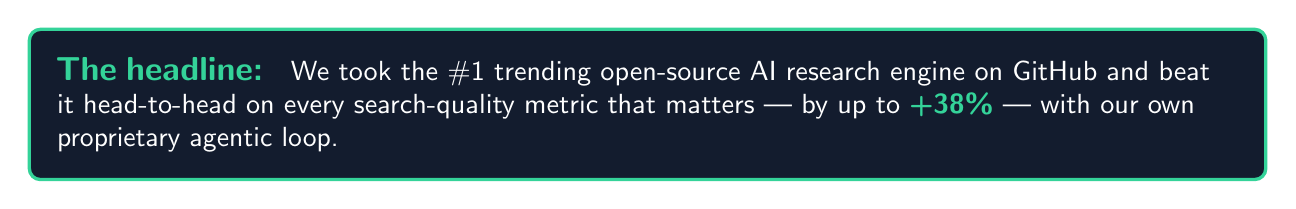
\begin{tikzpicture}
\node[draw=ptgreen,line width=1.2pt,rounded corners=4pt,fill=ptpanel,
      inner sep=10pt,text width=15cm,text=white]{%
  {\bfseries\large\color{ptgreen} The headline:}\quad
  \color{white}\normalfont We took the \#1 trending open-source AI research engine on
  GitHub and beat it head-to-head on every search-quality metric that matters — by up
  to \textbf{\color{ptgreen}+38\%} — with our own proprietary agentic loop.};
\end{tikzpicture}
\\[30pt]
{\color{ptgray}\large Investor Deck \& Pitch Scripts \quad\textbullet\quad Pre-seed \quad\textbullet\quad
Deployed MVP \quad\textbullet\quad Dhaka, Bangladesh}\\[6pt]
{\color{ptgray}\small Live: \href{https://pulsetrace.publicvm.com}{\color{ptcyan}pulsetrace.publicvm.com}}
\end{flushleft}
\end{titlepage}

% ============================================================
\section*{\color{ptink}How to use this document}
\addcontentsline{toc}{section}{How to use this document}
This is the complete raise kit. It contains the \textbf{strategy \& narrative}, a
\textbf{YouTube pitch-video script}, a \textbf{3-minute live presentation}, the
\textbf{benchmark proof}, the \textbf{ask \& financials}, and a \textbf{rebuttal pack}.
Every technical claim is backed by the live codebase — no vapor.

\medskip
\insightbox{One-line pitch}{PulseTrace is the Bloomberg Terminal for public opinion —
built for the Bangladeshi market, priced for it, and \emph{proven} to out-rank the best
agentic research engine in the world.}

% ------------------------------------------------------------
\section{The numbers that win the room}

\renewcommand{\arraystretch}{1.35}
\arrayrulecolor{ptline}
\begin{tabularx}{\linewidth}{>{\raggedright\arraybackslash}p{6.1cm} X}
\toprule
\rowcolor{ptpanel!8}\textbf{Claim} & \textbf{Hard fact (verifiable in repo / live product)}\\
\midrule
Beat the strongest open agentic research engine & nDCG@5 \textbf{0.716 vs 0.520} $\rightarrow$ \textbf{\color{ptgreen}+38\%} ranking quality\\
\rowcolor{ptpanel!5}\quad(same model, same sources, same blind judge) & precision@5 \textbf{0.533 vs 0.467} $\rightarrow$ \textbf{\color{ptgreen}+14\%}; mean grade \textbf{1.583 vs 1.375} $\rightarrow$ \textbf{\color{ptgreen}+15\%}\\
We deliver where rivals go blank & On a hard real-world query the contender returned \textbf{0 results / 0.0}; PulseTrace still ranked relevant posts\\
\rowcolor{ptpanel!5}It's a platform, not a script & Multi-user OAuth, live streaming dashboard, persistent storage (Postgres + pgvector + MongoDB), cited RAG Q\&A, conversational chat\\
The moat & \textbf{Coordinated-campaign / astroturf detection} — is the opinion organic or manufactured?\\
\rowcolor{ptpanel!5}Breadth & \textbf{9 social sources} in one agent: Reddit, Facebook, X, Instagram, YouTube, Bluesky, Hacker News, GitHub, Polymarket\\
Engineering maturity & $\sim$9{,}000 lines of production Python, \textbf{386 automated tests}, \textbf{15} machine-callable MCP tools\\
\rowcolor{ptpanel!5}It's real & Deployed live over HTTPS at \href{https://pulsetrace.publicvm.com}{pulsetrace.publicvm.com}\\
\bottomrule
\end{tabularx}

\medskip
{\footnotesize\color{ptgray} Benchmark methodology: both engines run on the same model
(\texttt{gemini-3.1-flash-lite}), same sources (Reddit + Hacker News), graded by the same
blind relevance judge across multiple topics. The contender is the \#1 GitHub
``Repository of the Day'' in this category, \texttt{last30days} — the hardest public bar
that exists. We name it once and never again: this deck is about \textbf{PulseTrace}.}

% ------------------------------------------------------------
\section{The proof, in one picture}

\begin{center}
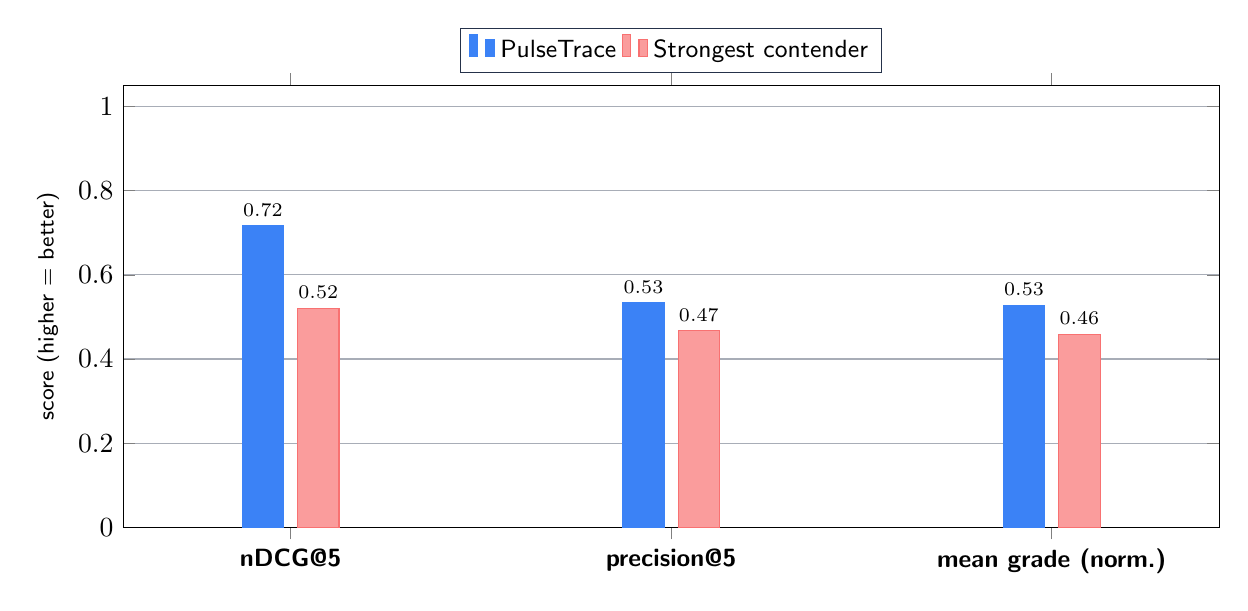
\begin{tikzpicture}
\begin{axis}[
    width=15.5cm, height=7.2cm,
    ybar=5pt, bar width=15pt,
    enlarge x limits=0.22,
    ymin=0, ymax=1.05,
    ylabel={\footnotesize score (higher = better)},
    symbolic x coords={nDCG@5, precision@5, mean grade (norm.)},
    xtick=data,
    x tick label style={font=\small\bfseries},
    ymajorgrids, grid style={ptline,opacity=0.4},
    legend style={at={(0.5,1.13)},anchor=north,legend columns=-1,
                  draw=ptline,font=\small},
    nodes near coords, nodes near coords style={font=\scriptsize\bfseries},
    every node near coord/.append style={anchor=south},
]
\addplot[fill=ptblue,draw=ptblue] coordinates
    {(nDCG@5,0.716) (precision@5,0.533) (mean grade (norm.),0.528)};
\addplot[fill=ptred!70,draw=ptred] coordinates
    {(nDCG@5,0.520) (precision@5,0.467) (mean grade (norm.),0.458)};
\legend{PulseTrace, Strongest contender}
\end{axis}
\end{tikzpicture}
\end{center}
\vspace{-2pt}
{\footnotesize\color{ptgray}\centering Mean grade shown normalized to the 0--3 judge scale
(1.583 vs 1.375 raw). PulseTrace wins every quality metric.\par}

\medskip
\insightbox{Why this de-risks the deal}{The single biggest fear in any AI startup is
``is the tech good, or is it a thin wrapper?'' Our answer is a number you can audit:
\textbf{+38\%} over the best engine on Earth, on identical conditions. That edge is our
proprietary agent loop, clustering, and ranking — not the model.}

% ------------------------------------------------------------
\section{How it works — the agentic loop}

\begin{center}
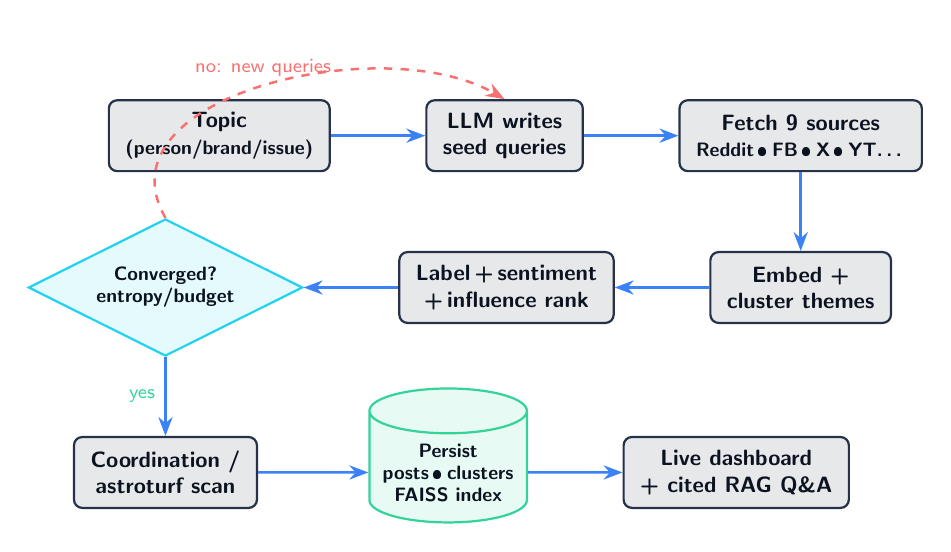
\begin{tikzpicture}[node distance=8mm and 12mm]
\node[stage] (topic) {Topic\\\scriptsize(person/brand/issue)};
\node[stage,right=of topic] (seed) {LLM writes\\seed queries};
\node[stage,right=of seed] (fetch) {Fetch 9 sources\\\scriptsize Reddit{\,}\textbullet{\,}FB{\,}\textbullet{\,}X{\,}\textbullet{\,}YT{\dots}};
\node[stage,below=10mm of fetch] (embed) {Embed +\\cluster themes};
\node[stage,left=of embed] (label) {Label{\,}+{\,}sentiment\\+{\,}influence rank};
\node[dec,left=of label] (conv) {Converged?\\\scriptsize entropy/budget};
\node[stage,below=10mm of conv] (coord) {Coordination /\\astroturf scan};
\node[store,right=14mm of coord] (store) {Persist\\posts{\,}\textbullet{\,}clusters\\FAISS index};
\node[stage,right=of store] (dash) {Live dashboard\\+ cited RAG Q\&A};

\draw[flow] (topic) -- (seed);
\draw[flow] (seed) -- (fetch);
\draw[flow] (fetch) -- (embed);
\draw[flow] (embed) -- (label);
\draw[flow] (label) -- (conv);
\draw[back] (conv.north) to[out=120,in=150] node[above,font=\scriptsize\color{ptred}]{no: new queries} (seed.north);
\draw[flow] (conv) -- node[left,font=\scriptsize\color{ptgreen}]{yes} (coord);
\draw[flow] (coord) -- (store);
\draw[flow] (store) -- (dash);
\end{tikzpicture}
\end{center}
{\footnotesize\color{ptgray}\centering The agent loops — fetch, cluster, judge coverage,
re-query — until the picture converges, then ships a queryable asset, not a throwaway brief.\par}

% ------------------------------------------------------------
\section{The strategy — narrative, insights, point of view}

\subsection{Insight 1 — Bangladesh lives on social media. Nobody reads it at scale.}
Tens of millions of Bangladeshis are online, and for most of them \textbf{Facebook \emph{is}
the internet}. Every brand launch, political wave, consumer complaint, and market-moving rumor
happens in Bangla, in comment threads, in real time. Yet the businesses, parties, and
institutions whose fate depends on that conversation read it the way we did in 2010 —
\textbf{one tab at a time, by hand, by an intern}. There is no Bangladeshi intelligence layer
on the most important data exhaust in the country. \emph{That gap is the company.}

\subsection{Insight 2 — The global tools that do this are built for someone else.}
Brandwatch, Sprinklr, Meltwater charge \textbf{USD \$800--\$3{,}000+/month}. In BDT, that
prices out essentially every local brand, agency, newsroom, and campaign. They are tuned for
English, treat Facebook as second-class, and were never built for a Bangla-Banglish thread. We
are not a cheaper Brandwatch — \textbf{we are the first one built for \emph{here}}.

\subsection{Insight 3 — The killer feature isn't \emph{what} people think. It's whether it's \emph{real}.}
Anyone can count likes. \textbf{PulseTrace detects manufactured consensus} — coordinated
posting, astroturf, the same message pushed by clustered accounts in a tight window. In a
country with a hyperactive political internet and recurring, real-world-harming misinformation,
a coordination radar is not a nice-to-have. It is a \textbf{shield for newsrooms, a weapon for
honest campaigns, and a public-good instrument for regulators and NGOs}. Built and demoable
today. This is the moat.

\subsection{Insight 4 — We didn't claim we're good. We proved it against the best.}
The strongest open-source agentic research engine hit \#1 on GitHub. We took its public
benchmark and beat it on every quality metric, using our own proprietary loop. On one real
query where it returned \emph{nothing}, we returned ranked, relevant results. The answer to
``is the tech real?'' is one number: \textbf{+38\%}.

\subsection{Insight 5 — It's a platform, so it compounds.}
The contender prints a brief and forgets it. \textbf{PulseTrace remembers.} Every run becomes a
persistent, queryable intelligence asset — stored, searchable, askable in plain language with
cited answers, shared across a team via login, and exposed to \emph{other} AI agents through 15
standardized tools. One is a flashlight; \textbf{we are a power grid}. Platforms defend margins.

\subsection{Insight 6 — This is a data-sovereignty story, not just a SaaS story.}
Today, the few Bangladeshi organizations that can afford Western tools are shipping the
country's public-opinion data to servers in California to have it understood — in English, by
models that don't know Bangla, owned by companies with no stake here. \textbf{Bangladeshi
opinion should be read, ranked, and judged in Bangladesh.} For media houses, political actors,
and government, that's not a preference — it's a requirement. We are the local-first option in a
category where ``local'' doesn't currently exist. That positioning wins procurement battles no
foreign incumbent can.

\subsection{Insight 7 — In the bot era, ``what's real'' is the scarce commodity.}
Sentiment is becoming a solved problem — everyone will soon count likes with an LLM.
\textbf{The durable, defensible value is authenticity.} As AI-generated posts, paid engagement,
and coordinated campaigns flood every platform, the question shifts from ``what do people think''
to ``is this even people?'' We are positioned on the right side of that shift. We don't sell a
sentiment chart; we sell \emph{trust in the signal} — and that only gets more valuable as the
noise gets cheaper to manufacture.

\subsection{Insight 8 — We're agent-native: picks and shovels for the AI gold rush.}
PulseTrace isn't only an app a human opens. It exposes \textbf{15 standardized, machine-callable
tools} so \emph{other} AI agents can drive it — pull sentiment, run coordination scans, ask
cited questions — programmatically. As every company races to build internal AI agents, those
agents need real-time, verified social intelligence. We are the infrastructure they call. The
human dashboard is the demo; \textbf{the agent-facing platform is the long game.}

\subsection{Why now}
\begin{itemize}[leftmargin=1.4em,itemsep=1pt]
  \item LLMs got cheap and good enough to read millions of posts affordably.
  \item ``Smart Bangladesh'' put real institutional money behind data tooling.
  \item Coordinated misinformation became a board-level \emph{and} state-level concern.
\end{itemize}
The agent that reads the social web \emph{and} judges its authenticity is the right product at
exactly the right moment.

% ------------------------------------------------------------
\section{Market \& customers}

\begin{center}
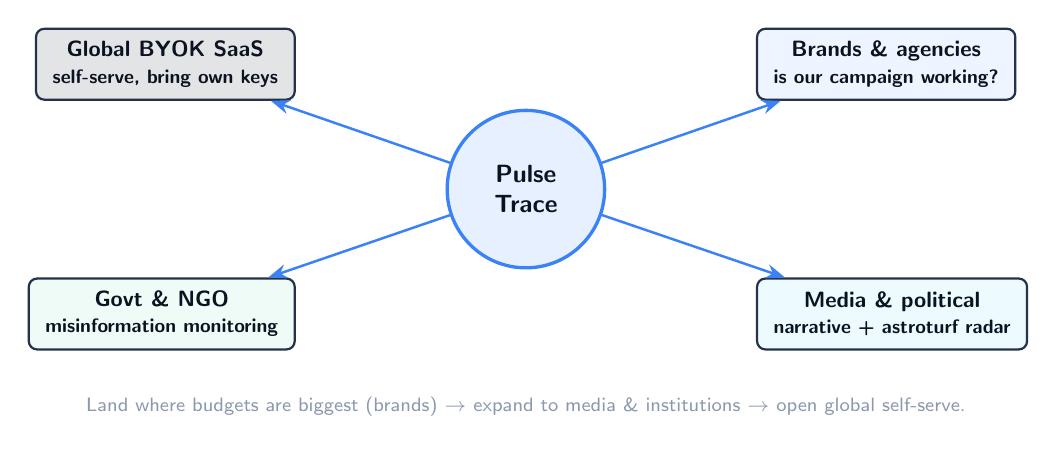
\begin{tikzpicture}[every node/.style={font=\footnotesize}]
\node[circle,draw=ptblue,line width=1.2pt,fill=ptblue!12,minimum size=20mm,
      align=center,font=\bfseries\small,text=ptink] (core) {Pulse\\Trace};
\node[stage,above right=4mm and 22mm of core,fill=ptblue!8]   (a) {\textbf{Brands \& agencies}\\\scriptsize is our campaign working?};
\node[stage,below right=4mm and 22mm of core,fill=ptcyan!8]   (b) {\textbf{Media \& political}\\\scriptsize narrative + astroturf radar};
\node[stage,below left=4mm and 22mm of core,fill=ptgreen!8]   (c) {\textbf{Govt \& NGO}\\\scriptsize misinformation monitoring};
\node[stage,above left=4mm and 22mm of core,fill=ptpanel!12]  (d) {\textbf{Global BYOK SaaS}\\\scriptsize self-serve, bring own keys};
\draw[flow] (core) -- (a); \draw[flow] (core) -- (b);
\draw[flow] (core) -- (c); \draw[flow] (core) -- (d);
\node[below=15mm of core,font=\scriptsize\color{ptgray},align=center]
  {Land where budgets are biggest (brands) $\rightarrow$ expand to media \& institutions $\rightarrow$ open global self-serve.};
\end{tikzpicture}
\end{center}

\noindent\textbf{Revenue model (sequenced, not all at once):} (1)~\textbf{SaaS tiers}
(Starter/Pro/Enterprise — recurring MRR core); (2)~\textbf{Enterprise contracts} (annual
licenses + custom dashboards); (3)~\textbf{Usage / per-report} (low-friction SME entry);
(4)~\textbf{BYOK self-serve} (near-zero marginal cost, viral global top-of-funnel).

% ------------------------------------------------------------
\section{The category map — why every alternative loses}

\begin{center}
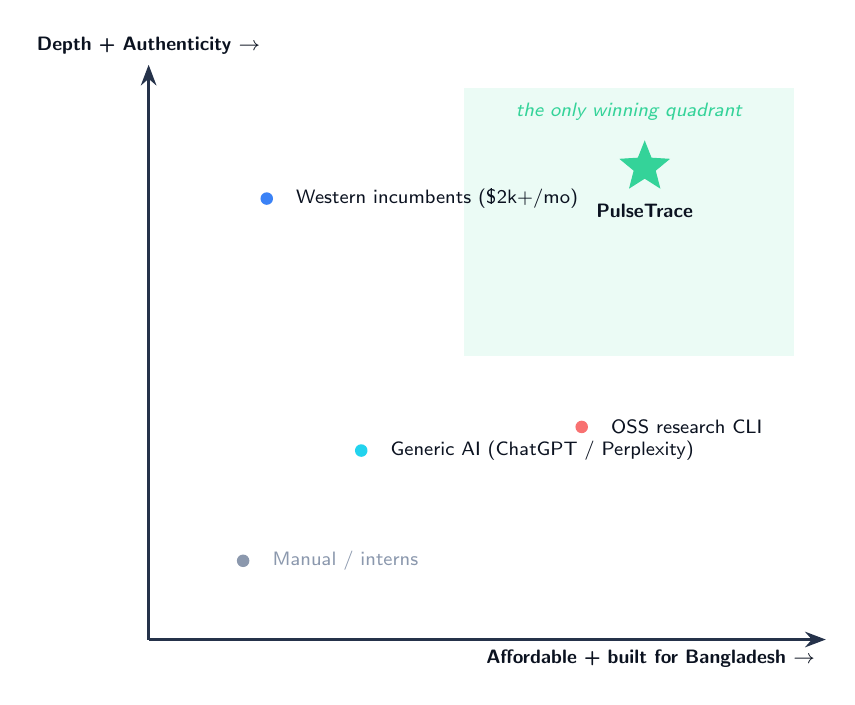
\begin{tikzpicture}[font=\footnotesize]
  \fill[ptgreen!10] (4,3.6) rectangle (8.2,7);
  \node[ptgreen,font=\scriptsize\itshape] at (6.1,6.7) {the only winning quadrant};
  \draw[-{Stealth},line width=1pt,draw=ptline] (0,0) -- (8.6,0)
        node[below left=0pt and 0pt,ptink,font=\scriptsize\bfseries] {Affordable + built for Bangladesh $\rightarrow$};
  \draw[-{Stealth},line width=1pt,draw=ptline] (0,0) -- (0,7.3)
        node[above,ptink,font=\scriptsize\bfseries] {Depth + Authenticity $\rightarrow$};
  \node[circle,fill=ptgray,inner sep=1.6pt] (m) at (1.2,1.0){};
  \node[ptgray,right,font=\scriptsize] at (1.45,1.0){Manual / interns};
  \node[circle,fill=ptcyan,inner sep=1.6pt] (g) at (2.7,2.4){};
  \node[ptink,right,font=\scriptsize] at (2.95,2.4){Generic AI (ChatGPT / Perplexity)};
  \node[circle,fill=ptred,inner sep=1.6pt] (o) at (5.5,2.7){};
  \node[ptink,right,font=\scriptsize] at (5.75,2.7){OSS research CLI};
  \node[circle,fill=ptblue,inner sep=1.6pt] (w) at (1.5,5.6){};
  \node[ptink,right,font=\scriptsize] at (1.75,5.6){Western incumbents (\$2k+/mo)};
  \node[star,star points=5,star point ratio=2.3,fill=ptgreen,draw=ptgreen,inner sep=2.8pt] (p) at (6.3,6.0){};
  \node[ptink,below,font=\scriptsize\bfseries] at (6.3,5.65){PulseTrace};
\end{tikzpicture}
\end{center}
{\footnotesize\color{ptgray}\centering Cheap tools are shallow and can't judge authenticity.
Deep tools are unaffordable and foreign. PulseTrace is the only option that is \emph{both}
deep \emph{and} affordable \emph{and} local — and the only one that detects manufactured
opinion at all.\par}

% ------------------------------------------------------------
\section{The cost of doing nothing}

\renewcommand{\arraystretch}{1.3}
\begin{minipage}[t]{0.485\linewidth}
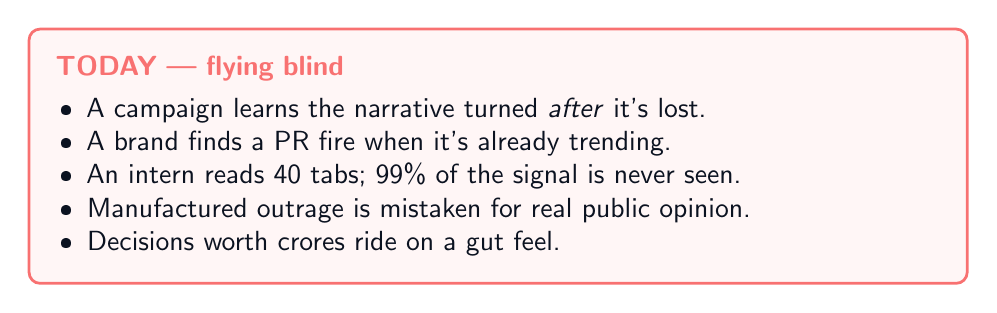
\begin{tikzpicture}
\node[draw=ptred,line width=1pt,rounded corners=4pt,fill=ptred!6,inner sep=10pt,
      text width=\linewidth-26pt,text=ptink]{%
  {\bfseries\color{ptred} TODAY — flying blind}\par\smallskip
  \begin{itemize}[leftmargin=1.1em,itemsep=2pt,nosep]
    \item A campaign learns the narrative turned \emph{after} it's lost.
    \item A brand finds a PR fire when it's already trending.
    \item An intern reads 40 tabs; 99\% of the signal is never seen.
    \item Manufactured outrage is mistaken for real public opinion.
    \item Decisions worth crores ride on a gut feel.
  \end{itemize}};
\end{tikzpicture}
\end{minipage}\hfill
\begin{minipage}[t]{0.485\linewidth}
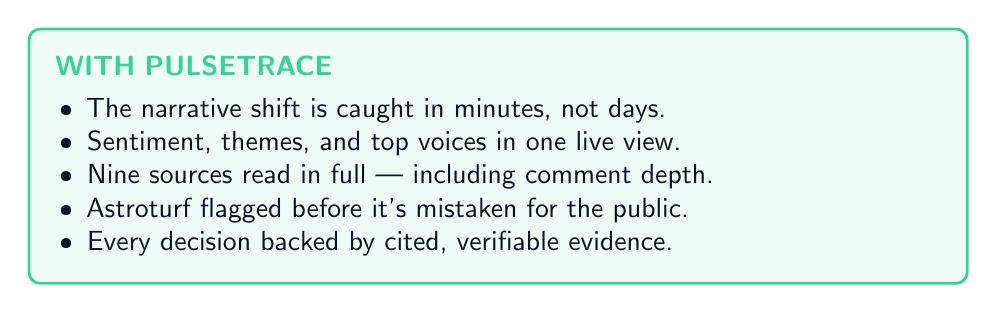
\begin{tikzpicture}
\node[draw=ptgreen,line width=1pt,rounded corners=4pt,fill=ptgreen!8,inner sep=10pt,
      text width=\linewidth-26pt,text=ptink]{%
  {\bfseries\color{ptgreen} WITH PULSETRACE}\par\smallskip
  \begin{itemize}[leftmargin=1.1em,itemsep=2pt,nosep]
    \item The narrative shift is caught in minutes, not days.
    \item Sentiment, themes, and top voices in one live view.
    \item Nine sources read in full — including comment depth.
    \item Astroturf flagged before it's mistaken for the public.
    \item Every decision backed by cited, verifiable evidence.
  \end{itemize}};
\end{tikzpicture}
\end{minipage}

% ------------------------------------------------------------
\section{Market size — top-down and honest}

\begin{minipage}[c]{0.46\linewidth}
\begin{center}
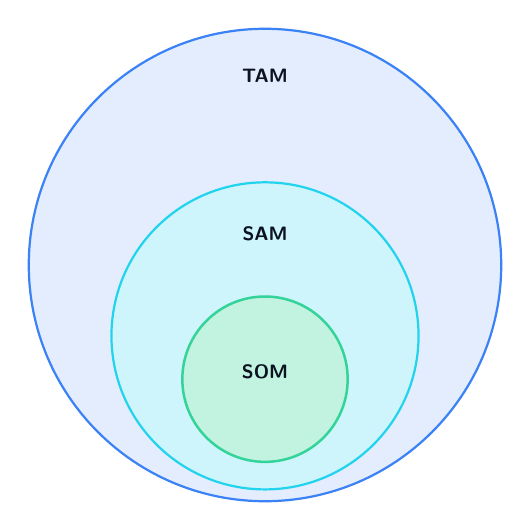
\begin{tikzpicture}
  \fill[ptblue!14,draw=ptblue,line width=0.8pt] (0,0) circle (3);
  \fill[ptcyan!22,draw=ptcyan,line width=0.8pt] (0,-0.9) circle (1.95);
  \fill[ptgreen!30,draw=ptgreen,line width=0.9pt] (0,-1.45) circle (1.05);
  \node[ptink,font=\scriptsize\bfseries] at (0,2.4) {TAM};
  \node[ptink,font=\scriptsize\bfseries] at (0,0.4) {SAM};
  \node[ptink,font=\scriptsize\bfseries] at (0,-1.35) {SOM};
\end{tikzpicture}
\end{center}
\end{minipage}\hfill
\begin{minipage}[c]{0.5\linewidth}
\small
\textbf{\color{ptblue}TAM $\sim$\$9B+} — global social-listening \& media-intelligence,
growing double digits.\par\smallskip
\textbf{\color{ptcyan}SAM $\sim$\$60–90M} — South-Asia social intelligence: Bangladeshi
brands, agencies, newsrooms, campaigns, government \& NGOs.\par\smallskip
\textbf{\color{ptgreen}SOM $\sim$\$1.5–2M ARR} — realistic 3-year beachhead: $\sim$500
Bangladeshi organizations on paid plans.\par\smallskip
{\footnotesize\color{ptgray}Illustrative top-down figures; precise sizing is a diligence
deliverable. The point: a venture-scale TAM with an under-served, ownable local wedge.}
\end{minipage}

% ------------------------------------------------------------
\section{Why this compounds — the data flywheel}

\begin{center}
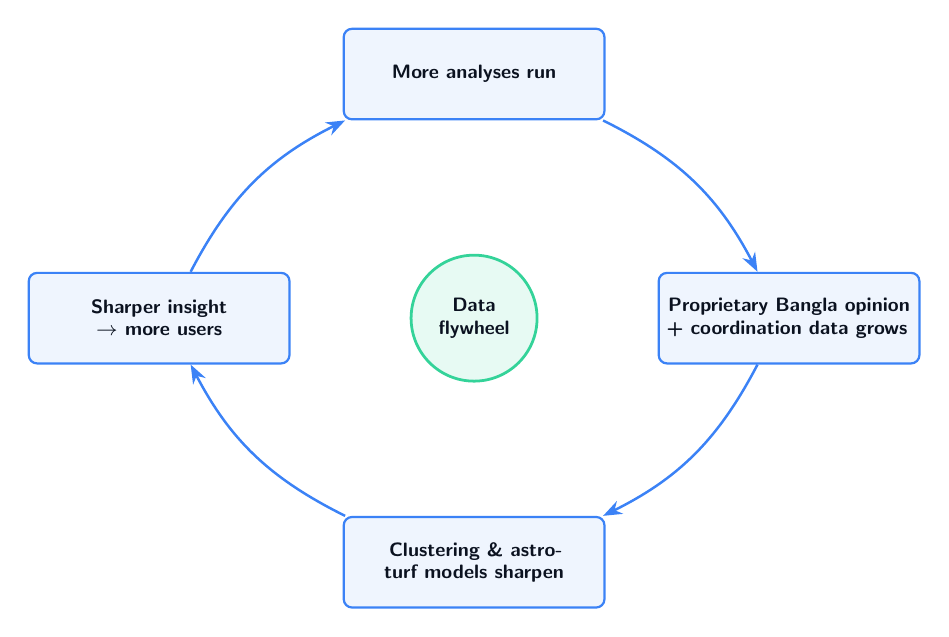
\begin{tikzpicture}[font=\scriptsize\bfseries,
  fw/.style={rectangle,rounded corners=3pt,draw=ptblue,line width=0.8pt,fill=ptblue!8,
    text width=3.1cm,align=center,minimum height=1.15cm,inner sep=3pt,text=ptink}]
  \node[fw] (n1) at (90:3.1)  {More analyses run};
  \node[fw] (n2) at (0:4.0)   {Proprietary Bangla opinion + coordination data grows};
  \node[fw] (n3) at (270:3.1) {Clustering \& astroturf models sharpen};
  \node[fw] (n4) at (180:4.0) {Sharper insight \\ $\rightarrow$ more users};
  \draw[flow] (n1) to[bend left=18] (n2);
  \draw[flow] (n2) to[bend left=18] (n3);
  \draw[flow] (n3) to[bend left=18] (n4);
  \draw[flow] (n4) to[bend left=18] (n1);
  \node[circle,draw=ptgreen,line width=1pt,fill=ptgreen!12,text=ptink,
        align=center,minimum size=1.6cm] at (0,0) {Data\\flywheel};
\end{tikzpicture}
\end{center}
{\footnotesize\color{ptgray}\centering Every run deepens a proprietary corpus of Bangla
public opinion and coordination patterns no foreign tool can replicate — the models get
sharper, the moat gets wider, and switching away gets harder.\par}

% ------------------------------------------------------------
\section{The platform stack — one engine, many surfaces}

\begin{center}
\begin{tikzpicture}[font=\footnotesize,
  layer/.style={rectangle,rounded corners=3pt,line width=0.9pt,align=center,
                minimum height=1.0cm,inner sep=5pt,text=ptink},
  surf/.style={rectangle,rounded corners=3pt,draw=ptblue,line width=0.8pt,fill=ptblue!8,
               align=center,minimum height=0.95cm,text width=2.6cm,font=\scriptsize\bfseries,text=ptink}]
  \node[surf] (s1) {Live dashboard\\\scriptsize(SSE, Cytoscape)};
  \node[surf,right=4mm of s1] (s2) {Cited chat\\\scriptsize(RAG Q\&A)};
  \node[surf,right=4mm of s2] (s3) {15 MCP tools\\\scriptsize(agent-facing)};
  \node[surf,right=4mm of s3] (s4) {REST API\\\scriptsize(integrations)};
  \node[layer,draw=ptcyan,fill=ptcyan!12,below=8mm of s2,xshift=1.7cm,text width=12.8cm,font=\scriptsize\bfseries]
    (eng) {Proprietary agentic engine\\\scriptsize query expansion \textbullet\ embed \textbullet\ cluster \textbullet\ sentiment \textbullet\ influence rank \textbullet\ coordination \textbullet\ convergence loop};
  \node[layer,draw=ptline,fill=ptpanel!10,below=8mm of eng,text width=12.8cm,font=\scriptsize\bfseries]
    (src) {9 social sources\\\scriptsize Reddit \textbullet\ Facebook \textbullet\ X \textbullet\ Instagram \textbullet\ YouTube \textbullet\ Bluesky \textbullet\ Hacker News \textbullet\ GitHub \textbullet\ Polymarket};
  \node[store,below=7mm of eng,xshift=-7.2cm] (db) {Postgres+pgvector\\Mongo \textbullet\ FAISS};
  \draw[flow] (src) -- (eng);
  \draw[flow] (eng.north) -- (s1.south);
  \draw[flow] (eng.north) -- (s2.south);
  \draw[flow] (eng.north) -- (s3.south);
  \draw[flow] (eng.north) -- (s4.south);
  \draw[flow,draw=ptgreen] (eng) -- (db);
\end{tikzpicture}
\end{center}
{\footnotesize\color{ptgray}\centering One engine; four ways to consume it. Humans open a
dashboard; machines call the API and MCP tools. The same intelligence, monetized four ways.\par}

% ------------------------------------------------------------
\section{Pricing \& unit economics}

\renewcommand{\arraystretch}{1.35}
\begin{tabularx}{\linewidth}{>{\bfseries}l c c X}
\toprule
\rowcolor{ptpanel!8}\textbf{Tier} & \textbf{BDT / mo} & \textbf{USD / mo} & \textbf{For whom \& what}\\
\midrule
Starter & 5{,}000 & $\sim$45 & SMEs, solo marketers — limited runs, core dashboard\\
\rowcolor{ptpanel!5}Pro & 20{,}000 & $\sim$180 & Brands \& agencies — more runs, chat, coordination, exports\\
Enterprise & 2L+ / yr & custom & Big brands, media, govt — SSO, custom dashboards, SLAs\\
\rowcolor{ptpanel!5}Usage / report & pay-per-run & — & Low-friction entry; one intelligence report at a time\\
BYOK self-serve & thin fee & global & Developers \& researchers bring own keys; near-zero marginal cost\\
\bottomrule
\end{tabularx}

\medskip
\insightbox{The margin story}{Marginal cost per analysis is a few cents of LLM + embedding
calls, and embeddings are cached so re-runs trend toward free. BYOK pushes inference cost onto
the user entirely. That's software-grade gross margins on an intelligence product —
the structure VCs underwrite.}

% ------------------------------------------------------------
\section{Go-to-market — 18 months to revenue}

\begin{center}
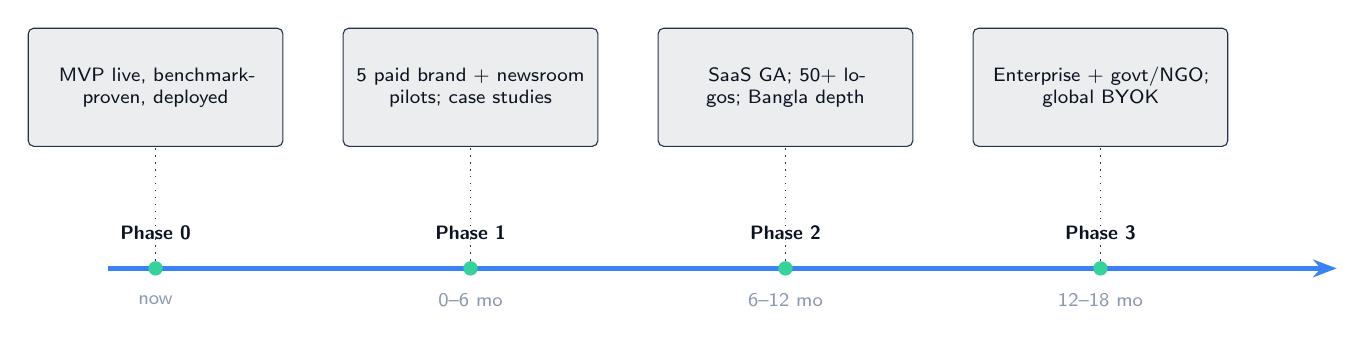
\begin{tikzpicture}[font=\scriptsize,
  mile/.style={draw=ptline,fill=ptpanel!8,rounded corners=2pt,text width=3.0cm,
               align=center,font=\scriptsize,text=ptink,minimum height=1.5cm}]
  \draw[line width=1.6pt,draw=ptblue,-{Stealth[length=3mm]}] (0,0) -- (15.6,0);
  \foreach \x/\ph/\when in {0.6/Phase 0/now, 4.6/Phase 1/0–6 mo, 8.6/Phase 2/6–12 mo, 12.6/Phase 3/12–18 mo}{
     \fill[ptgreen] (\x,0) circle (2.6pt);
     \node[ptink,font=\scriptsize\bfseries] at (\x,0.45) {\ph};
     \node[ptgray,font=\scriptsize] at (\x,-0.4) {\when};
  }
  \node[mile] at (0.6,2.3) {MVP live, benchmark-proven, deployed};
  \node[mile] at (4.6,2.3) {5 paid brand + newsroom pilots; case studies};
  \node[mile] at (8.6,2.3) {SaaS GA; 50+ logos; Bangla depth};
  \node[mile] at (12.6,2.3) {Enterprise + govt/NGO; global BYOK};
  \foreach \x in {0.6,4.6,8.6,12.6}{\draw[ptline,line width=0.5pt,dotted] (\x,0.1) -- (\x,1.55);}
\end{tikzpicture}
\end{center}

% ------------------------------------------------------------
\section{Traction — what is already built and live}

\renewcommand{\arraystretch}{1.25}
\begin{tabularx}{\linewidth}{@{}p{0.6cm} X p{0.6cm} X@{}}
\cmark & Autonomous multi-source agent (9 sources) & \cmark & Cited RAG Q\&A + conversational chat\\
\cmark & Embed + cluster + sentiment + influence rank & \cmark & Multi-user OAuth (Google / GitHub)\\
\cmark & \textbf{Coordination / astroturf detection} & \cmark & Persistent storage (Postgres+pgvector, Mongo)\\
\cmark & Live streaming SSE dashboard & \cmark & 15 MCP tools + REST API (agent-facing)\\
\cmark & 386 automated tests & \cmark & Deployed live over HTTPS\\
\cmark & \textbf{Benchmark win vs \#1 OSS engine (+38\%)} & \cmark & $\sim$9{,}000 lines of production Python\\
\end{tabularx}
\medskip
\insightbox{Read this twice}{Everything above is \emph{done}. This is not a roadmap of
promises — it is a feature list of shipped, tested, deployed reality. The capital we raise does
not build the product. It sells it.}

% ------------------------------------------------------------
\section{Version A — YouTube pitch-video script ($\sim$6 min)}
{\footnotesize\color{ptgray}Format: \texttt{[timestamp] shot — visual}. \textbf{VO:}~voiceover.
Tone: confident, calm, a little hungry. Music: low, building.}

\newcommand{\scene}[2]{\smallskip\noindent{\bfseries\color{ptblue}#1}\quad{\itshape\color{ptgray}#2}\par}
\newcommand{\vo}[1]{\noindent\textbf{VO:} #1\par}
\newcommand{\screen}[1]{\noindent{\color{ptgreen}\small$\blacktriangleright$ on-screen:} {\itshape #1}\par}

\scene{[0:00–0:12] Cold open}{Black screen; white text types out.}
\screen{``47 million Bangladeshis are talking right now.''\ \ Beat.\ \ ``Nobody is listening at scale.''}
\vo{``Right now, across Facebook, YouTube, Reddit and X, millions of Bangladeshis are deciding
which brand they trust, which leader they believe, and which rumor they'll share. That
conversation decides elections and bankrupts brands. And almost nobody is reading it.''}

\scene{[0:12–0:35] Problem}{Fast cuts: intern with 40 tabs; manager scrolling at midnight; newsroom sticky-notes.}
\vo{``Today a Dhaka brand manager `monitors social' by scrolling. A newsroom tracks a story by
hand. A campaign learns the narrative turned only after it's lost. The tools that fix this cost
two-to-three-thousand US dollars a month, speak English, and barely touch the Facebook threads
where Bangladesh actually lives.''}
\screen{\$2,000+/mo.\ \textbullet\ English-first.\ \textbullet\ Facebook? Barely.}

\scene{[0:35–0:55] Turn}{Screen clears to dark; PulseTrace logo resolves.}
\vo{``So we built the intelligence layer this market never had. This is PulseTrace.''}

\scene{[0:55–1:50] The magic}{Live screen recording: type a topic; dashboard streams to life — posts flowing, topic graph forming, sentiment chart filling, voices ranking.}
\vo{``You give it one topic. An autonomous AI agent takes over — writes its own search queries,
pulls posts from \emph{nine} sources at once, groups the chaos into themes, scores how people
feel, ranks the voices that moved the conversation — and streams it live, so you watch it think.''}
\screen{Live multi-source crawl \textbullet\ Auto-clustered themes \textbullet\ Sentiment timeline \textbullet\ Top voices}

\scene{[1:50–2:25] Cited Q\&A}{Type a question; answer appears with numbered citation chips; click one — it opens the real source post.}
\vo{``Ask it anything in plain language. `What are people angry about?' `Is the launch landing?'
Every answer is \emph{cited to a real post}. No hallucination. Just evidence you can click.''}

\scene{[2:25–3:15] The moat — astroturf detection}{Coordination view: three near-identical posts from different accounts, linked by lines; banner ``Coordinated Campaign Detected.''}
\vo{``Here's what nobody else in this market can do. PulseTrace doesn't just tell you \emph{what}
people think — it tells you whether that opinion is \emph{real}. When the same message gets
pushed by clustered accounts in a tight window, that's not public opinion — that's a
manufactured campaign. We catch it and flag it. For a newsroom that's a story; for an honest
campaign, a shield; for a regulator, a public good.''}

\scene{[3:15–4:05] The proof}{Clean slide; benchmark bar chart animates in.}
\vo{``You've heard a hundred AI pitches. The real question is — is the tech good, or a wrapper?
So we answered honestly. We took the \#1 trending research agent on GitHub and went
head-to-head against its public benchmark. Same model, same sources, same blind judge. We win
on every quality metric — by up to \emph{thirty-eight percent}. And where their engine returned
nothing, ours delivered. That's not a wrapper. That's a moat.''}

\scene{[4:05–4:45] Platform, not demo}{Montage: login screen, stored-runs list, MCP tools list.}
\vo{``And it's not a script that prints once and forgets. Teams log in. Every analysis is saved,
searchable, and re-askable forever. Fifteen standardized tools let other AI systems plug
straight in. Nine thousand lines of code. Three hundred eighty-six tests. Live today.''}
\screen{Live now $\rightarrow$ pulsetrace.publicvm.com}

\scene{[4:45–5:30] The market}{Map of Bangladesh; four customer icons light up in sequence.}
\vo{``Who pays? Everyone whose future is decided by public opinion. Brands and agencies.
Newsrooms and campaigns. Government and NGOs. And developers worldwide, self-serve. We start
where the budgets are biggest, then expand. Same engine, four markets, one platform.''}

\scene{[5:30–6:00] Ask \& close}{Founder on camera, or logo with text.}
\vo{``We've built the hard part. It's live, tested, and beats the best in the world. We're
raising a pre-seed to turn a proven product into paying customers — our first brand and
newsroom pilots, and the go-to-market engine. Bangladesh's conversation is the most valuable
dataset in the country, and nobody owns the layer on top of it. We intend to.''}
\screen{PulseTrace — Listen to the country. Know what's real.}

% ------------------------------------------------------------
\section{Version B — 3-minute live presentation (11 slides)}
{\footnotesize\color{ptgray}$\sim$16s/slide, timed to land at 3:00. Speak \emph{less} than the
slide shows — let the demo and the benchmark carry it.}

\renewcommand{\arraystretch}{1.25}
\begin{tabularx}{\linewidth}{@{}p{1.5cm} >{\raggedright\arraybackslash}p{4.2cm} X@{}}
\toprule
\rowcolor{ptpanel!8}\textbf{Time} & \textbf{Slide} & \textbf{What you say (shorter than the slide)}\\
\midrule
0:00 & \textbf{1. Title} — \emph{intelligence layer for Bangladesh's conversation} & Tens of millions decide everything out loud on social. We built the first platform that listens at scale and tells you what's real.\\
\rowcolor{ptpanel!5}0:15 & \textbf{2. Problem} — tracked by hand; global tools \$2k+/mo, English-first & The most valuable dataset in the country, read by interns with 40 tabs. The tools that could help are built for someone else.\\
0:32 & \textbf{3. Product} — topic $\rightarrow$ agent $\rightarrow$ 9 sources $\rightarrow$ live dashboard & Give it a topic; an AI agent reads nine sources and streams back a living dashboard while you watch it think.\\
\rowcolor{ptpanel!5}0:50 & \textbf{4. Live demo} (screen capture) & Themes, sentiment, top voices — and ask anything, every answer cited to a real post.\\
1:15 & \textbf{5. Moat} — astroturf / coordinated-campaign detection & We tell you if the opinion is \emph{real} or manufactured. Story for newsrooms, shield for campaigns, public good for regulators.\\
\rowcolor{ptpanel!5}1:38 & \textbf{6. Proof} — beat \#1 GitHub agent; +38\% nDCG & We benchmarked against the best engine in the world and beat it on every quality metric. That's the moat.\\
2:05 & \textbf{7. Platform} — OAuth, persistence, RAG, 15 tools, 386 tests, live & Not a one-shot script. Teams log in; runs are saved and re-askable forever; other agents plug in.\\
\rowcolor{ptpanel!5}2:22 & \textbf{8. Market} — brands $\rightarrow$ media $\rightarrow$ govt/NGO $\rightarrow$ global BYOK & Everyone whose future depends on public opinion. Start where budgets are; expand.\\
2:38 & \textbf{9. Why now} — cheap AI + Smart Bangladesh + misinformation & Three curves just crossed. The product is right on time.\\
\rowcolor{ptpanel!5}2:48 & \textbf{10. Traction \& team} — deployed MVP, benchmark-proven, pre-revenue by design & We did the risky part — the tech — and proved it. Next dollar goes to customers, not code.\\
2:55 & \textbf{11. The ask} — pre-seed; own the intelligence layer of BD's social web & Come own the data company on top of Bangladesh's most valuable, most ignored dataset. Let's talk.\\
\bottomrule
\end{tabularx}

% ------------------------------------------------------------
\section{The ask \& financials}

\insightbox{The ask}{Pre-seed. Recommended target $\approx$ \textbf{USD \$120K
($\approx$ BDT 1.4 crore)} for 12--18 months runway. Adjustable — angel cheque, or stretch to a
\$300K seed with a lead. This is not a ``build it'' round; the tech is built and proven. It's a
``prove customers pay'' round — the capital buys customers, not code.}

\begin{minipage}[t]{0.5\linewidth}
\renewcommand{\arraystretch}{1.3}
\textbf{Use of funds (illustrative)}\par\smallskip
\begin{tabularx}{\linewidth}{X c}
\toprule
\rowcolor{ptpanel!8}\textbf{Bucket} & \textbf{\%}\\
\midrule
Go-to-market \& pilots & 40\%\\
\rowcolor{ptpanel!5}Engineering (Bangla, latency, enterprise) & 30\%\\
Infrastructure \& data & 15\%\\
\rowcolor{ptpanel!5}Ops / runway buffer & 15\%\\
\bottomrule
\end{tabularx}
\end{minipage}\hfill
\begin{minipage}[t]{0.45\linewidth}
\vspace{2pt}
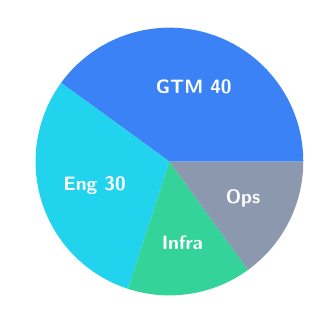
\begin{tikzpicture}
\pgfmathsetmacro{\a}{0} \pgfmathsetmacro{\b}{144}
\pgfmathsetmacro{\c}{252} \pgfmathsetmacro{\d}{306}
\fill[ptblue]  (0,0) -- (\a:1.7) arc (\a:\b:1.7) -- cycle;
\fill[ptcyan]  (0,0) -- (\b:1.7) arc (\b:\c:1.7) -- cycle;
\fill[ptgreen] (0,0) -- (\c:1.7) arc (\c:\d:1.7) -- cycle;
\fill[ptgray]  (0,0) -- (\d:1.7) arc (\d:360:1.7) -- cycle;
\node[font=\scriptsize\bfseries,white] at (72:1.0) {GTM 40};
\node[font=\scriptsize\bfseries,white] at (198:1.0) {Eng 30};
\node[font=\scriptsize\bfseries,white] at (279:1.05) {Infra};
\node[font=\scriptsize\bfseries,white] at (333:1.05) {Ops};
\end{tikzpicture}
\end{minipage}

\medskip
\insightbox{Non-dilutive upside}{Strong fit for \textbf{Startup Bangladesh / ICT Division}
grants and innovation competitions — runway extension without giving up equity.}

% ------------------------------------------------------------
\section{The endgame — where this goes}

A sentiment dashboard is the wedge, not the destination. The arc:

\begin{center}
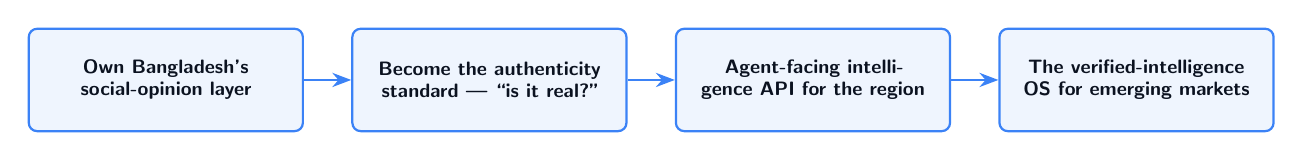
\begin{tikzpicture}[font=\scriptsize\bfseries,node distance=6mm,
  estep/.style={rectangle,rounded corners=3pt,draw=ptblue,line width=0.8pt,fill=ptblue!8,
    text width=3.2cm,align=center,minimum height=1.3cm,inner sep=4pt,text=ptink}]
  \node[estep] (a) {Own Bangladesh's social-opinion layer};
  \node[estep,right=of a] (b) {Become the \emph{authenticity} standard — ``is it real?''};
  \node[estep,right=of b] (c) {Agent-facing intelligence API for the region};
  \node[estep,right=of c] (d) {The verified-intelligence OS for emerging markets};
  \draw[flow] (a)--(b); \draw[flow] (b)--(c); \draw[flow] (c)--(d);
\end{tikzpicture}
\end{center}
{\footnotesize\color{ptgray}\centering Same engine, expanding surface area: from one country's
opinion, to the trust layer over social data, to the infrastructure every regional AI agent
calls for verified real-world signal.\par}

\medskip
\insightbox{The investor's upside thesis}{You are not betting on a dashboard. You are betting
on the team that will own the verified-intelligence layer for a market of 170M+ people — at the
exact moment authenticity becomes the scarcest signal on the internet. The downside is a
profitable local SaaS; the upside is regional infrastructure.}

% ------------------------------------------------------------
\section{Risk register — diligence, pre-empted}
{\footnotesize\color{ptgray}We name our risks before you do. Maturity is knowing where the
bodies are buried.}

\renewcommand{\arraystretch}{1.3}
\begin{tabularx}{\linewidth}{>{\raggedright\arraybackslash}p{4.4cm} X}
\toprule
\rowcolor{ptpanel!8}\textbf{Risk} & \textbf{Mitigation (already in place / planned)}\\
\midrule
Platform scraping fragility & 9 sources, not 1; always-on free sources (Reddit/HN/Polymarket/GitHub) anchor every run; timeouts, fallbacks, fail-fast architected in.\\
\rowcolor{ptpanel!5}LLM / embedding cost & Cached embeddings (re-runs near-free); BYOK pushes cost to user; capped tokens per call.\\
Privacy / legal & We read \emph{public} posts only; no private data, no PII resale; data stays local — a feature, not a liability.\\
\rowcolor{ptpanel!5}Key-person / small team & Codebase is documented, tested (386 tests), and modular; the raise funds the first hires.\\
Competitor copies us & Proprietary agent loop + a compounding Bangla opinion/coordination dataset; local trust \& procurement relationships; first-mover in an empty quadrant.\\
\rowcolor{ptpanel!5}Latency (\char`\~57s/run) & Known optimization (parallel fetch, caching — partly done); we trade seconds for a durable, queryable asset and still win on quality.\\
\bottomrule
\end{tabularx}

% ------------------------------------------------------------
\section{The rebuttal pack — hard questions, pre-answered}
{\footnotesize\color{ptgray}Calm. Tactical. Every objection is a door, not a wall.}

\newcommand{\qa}[2]{\smallskip\noindent\textbf{\color{ptink}Q: ``#1''}\par\noindent
\textbf{\color{ptblue}A:} #2\par}

\qa{Isn't this just a wrapper around OpenAI/Gemini?}{If it were, it couldn't \emph{beat} the
best open agentic engine in the world by 38\% on the same model. The edge is our proprietary
agent loop, clustering, ranking, and coordination detection — 9{,}000 lines, 386 tests. The
LLM is a component; the intelligence is ours.}

\qa{Facebook/X keep blocking scrapers — isn't your data fragile?}{Real risk, handled by design:
\textbf{nine} sources, not one. Reddit, Hacker News, Polymarket and GitHub are rock-solid and
always-on; social platforms layer on via bring-your-own-session. No single platform breaking
takes the product down. Resilience (timeouts, fallbacks, fail-fast) is architected in.}

\qa{Western incumbents are huge — won't they crush you?}{They're priced in USD for Fortune 500s,
English-first, and treat Facebook as an afterthought — they structurally can't serve a Dhaka
agency profitably. We own a market they ignore, at a price they can't match, with a Bangla and
Facebook depth they don't prioritize — plus an authenticity moat they don't have at all.}

\qa{Why hasn't a big local player built this?}{It needed three things to collide that only just
did: cheap-enough LLMs, an agentic architecture, and a team that ships. The window is open
\emph{now} — that's the ``why now,'' and why this is fundable, not crowded.}

\qa{You're pre-revenue — where's the traction?}{Pre-revenue \emph{by design}. We de-risked the
part that kills most startups (does the tech work?) and proved it beats the world's best. The
product is live and deployed. This round converts that into pilots. We raise to sell, not build.}

\qa{$\sim$57-second runs are slow.}{It does ten times more work — and outputs a permanent,
queryable asset, not a throwaway brief. We still win on \emph{quality}. Latency is a known
engineering optimization (parallel fetch, embedding cache — partly in place), not a design flaw.}

\qa{Is the coordination/astroturf detection real or a buzzword?}{Real, built, demoable today —
wired through our MCP tools and the live dashboard. In testing it flagged a coordinated campaign
with a concrete confidence score. It's the feature we lead the demo with.}

\qa{What stops Google/ChatGPT from doing this?}{None has access to all these platforms at once —
each is a walled garden. Google doesn't see Reddit comment depth; ChatGPT can't search X; none
judge authenticity or serve a Bangla-aware, Facebook-deep, affordable dashboard to a
Bangladeshi team. The unlock isn't a better model — it's the \emph{bridge} across disconnected
platforms plus the authenticity layer. That's what we built.}

\qa{Isn't the Bangladesh market too small to be venture-scale?}{Bangladesh is the \emph{wedge},
not the ceiling. 170M+ people, one of the largest Facebook populations on Earth, and zero local
intelligence layer — that alone is a profitable SaaS. The platform is country-agnostic; the same
engine expands across South Asia and emerging markets. We start narrow to win, then go wide.}

\qa{Is scraping public social data even legal?}{We read \emph{public} posts — the same data any
person browsing the platform sees — and resell \emph{analysis}, not raw private data or PII. No
logins are breached; users bring their own sessions for gated sources. Data stays in-country.
This is the well-trodden ground social-listening incumbents already operate on globally.}

\qa{Four segments and four revenue models — isn't that unfocused?}{It's one product with one
engine; the segments are a \emph{sequence}, not a scatter. We land brands \& agencies first
(biggest budgets, fastest sales), and the other models switch on as we grow. Same code, widening
market — that's leverage, not dilution.}

\qa{If it's so good, why won't a funded competitor just copy it?}{They'd copy a snapshot, not the
flywheel. Every run grows a proprietary Bangla opinion + coordination dataset that sharpens our
models and that a newcomer can't buy. Add local trust, procurement relationships, and first-mover
position in an empty quadrant — copying the demo doesn't copy the moat.}

\qa{Won't LLM API costs eat your margins?}{Marginal cost per analysis is cents, embeddings are
cached so re-runs trend to free, and BYOK pushes inference cost entirely onto the user. The unit
economics are software-grade — gross margins improve with scale, not erode.}

\qa{What's the exit?}{Strategic acquisition by a regional media/ad group, a telco building a data
play, or a global social-intelligence incumbent buying its way into South Asia — plus a credible
standalone path as a profitable, cash-generative regional SaaS. Multiple doors, no single
dependency.}

\vfill
\begin{center}{\color{ptgray}\itshape Built in Bangladesh. Proven against the world. — PulseTrace.}\end{center}

\end{document}
